
\chapter{Official Use of Nāgarī/Nandī Nāgarī South of Vindhya Scripts of One India}\label{chapter5}

\Authorline{Bimal Trivedi}


\section*{Abstract}

If Sanskrit is mother of many languages then Brāhmī\index{Brahmi@Brāhmī} is mother of almost all scripts used in India and many Asian / East Asian nations. Needless to mention that current “English Numerals” have directly Been derived from Brāhmī numerals,\index{numerals} hence Brāhmī is mother of modern numerals also.

Stone inscriptions\index{Stone inscriptions} of Ashoka,\index{Ashoka} found wide across India – from today’s Afghanistan (!) to Karnataka in further south and in the east; are ample proof that people knew how to read Brāhmī and the script was widely popular. The script was used with minor differences in curves and strokes, as the time and places changed. Tamil Brāhmī\index{Tamil Brahmi@Tamil Brāhmī} is not an exception. Brāhmī was a truly national script of ancient India. Brāhmī remained official script of mighty Mauryan,\index{Maurya} Satavahana,\index{Satavahana} Gupta\index{Gupta} and Harsha empires.\index{Harsha empires} It was well accepted official script with other small rulers and dynasties, viz., Western Kshatraps, Traikutaka, Rashtrakuta,\index{Rashtrakuta} Kidarites and many city states. Empires like Kushan,\index{Kushan} Sasankas, Palas\index{Pala} and invaders like Huns\index{Huns} gave it a deserved place in their administrative works. Two Indo-Greek rulers, named Agathocles and Pantaleon, minted coins with their names inscribed in Brāhmī in second century BCE along with Bactrian Greek. These bi-lingual / bi-script coins helped James Princep\index{Princep, James} to decipher Brāhmī.

Gupta Brāhmī is precursor of modern Nāgarī. However, later forms of Brāhmī are found till 8-9th century CE.

Likewise, Nāgarī was official script of mighty rulers and emperors of north and south of Vindhya, Sri Lanka was not an exception. South Indian emperors introduced Nāgarī\index{Nagari@Nāgarī} in Sri Lanka\index{Sri Lanka} and made it an official script beyond Kanyakumari.

Like Brāhmī, Nāgarī in various forms was used as official script on these rulers’ coins, copper plates and manuscripts. Starting clock-wise from far North-West Hindu Shahi rulers of today’s Afghanistan, Nāgarī was official script of Kashmir, Kangra, Nepal, Assam, Tripura and for a short period in Arakan. Pallavas,\index{Pallava} Cholas,\index{Chola} Vir Kerala\index{Vir Kerala} of Kerala, mighty Vijayanagara\index{Vijayanagara} rulers, Chhatrapati Shivaji,\index{Shivaji, Chhatrapati} Solankis\index{Solankis} of Gujarat, Chandelas,\index{Chandelas} Chauhans,\index{Chauhan} Parmars\index{Parmar} of middle and north India – made it a true pan Indian official script.

Characters of these two scripts were used by Indian people to write in one or more languages, each for thousand years, in East, West, North and South and South of South India.

This put to rest the notion that India never had one common script. Interestingly, this also throws light on common language/s, literacy, scholarly activities of the time and religiosity.


\section*{Brāhmī as One Script of Ancient India}

Since Nāgarī and other scripts of India have been derived from Brāhmī,\index{Brahmi@Brāhmī} studying the use of the Brāhmī around and south of Vindhyas will help in further understanding the spread of Nāgarī\index{Nagari@Nāgarī} and her sister scripts. Two significant places where many forms of Brāhmī have been etched in stone over many centuries and are preserved till date are worth mentioning:

\begin{enumerate}[{\rm 1)}]
\itemsep=0pt
\item Sanchi Stupa – Madhya Pradesh, Little North of Vindhya range

 \item Kanheri Caves – Borivali, Mumbai, Maharashtra

\end{enumerate}

The other places where Brāhmī inscriptions of historical importance are found, are, viz., Sopara, Junnar/Naneghat caves, Pandav Leni Caves, Bhaja caves, many places in Karnataka, Andhra Pradesh, Kerala and Brāhmī/Tamil Brāhmī in Tamil Nadu etcin Sanskrit, Pali and Prakrit languages.

Brāhmī diversified into many local scripts of South and South East Asia, which are known as Brāhmīc scripts. Thus Brāhmī was not just the mother of Indian scripts but world’s one of the most influential writing traditions. Thomas Trautman\index{Trautman, Thomas} claims that at least 198 scripts have derived from Brāhmī.

\subsection*{Sanchi Stupa Brāhmī Inscriptions}

Sanchi stupa was built by Emperor Ashoka\index{Ashoka} in 3rd century BCE. The stupa records numerous donations received from various people, rulers and emperors like Chandra Gupta Vikramaditya.\index{Vikramaditya, Chandra Gupta} These inscriptions are etched from 3rd Century BCE to 5-6th Century CE, for almost over thousand years and from people donating from almost across India. Most of the inscriptions are in Brāhmī of various forms and eras. Some inscriptions are found in Shankhānd Nāgarī\index{Shankhand Nagari@Shankhānd Nāgarī} script sharing space with Brāhmī. They are one sentence inscriptions giving names of donors etched on panels, architraves, walls and even on floors. 

Being a center of Buddhism, Sanchi attracted people from all the places, from east/west/south/north of India, irrespective of ethnicity, region or religious back ground of donors and visitors. Though, Sanchi is located little north of Vindhyas, it is in the middle - at the heart of India. Centrally located, Sanchi was a vibrant and most visited place as apparent from various panels, sculptures and versions of Brāhmī found there.

\textit{Example of Ashokan Brāhmī at Sanchi:}

Ashokan Brāhmī\index{Ashokan Brahmi@Ashokan Brāhmī} was widely used from 3rd Century BCE to 1st Century BCE, one such inscription in Ashokan Brāhmī:

\vskip 2pt

\centerline{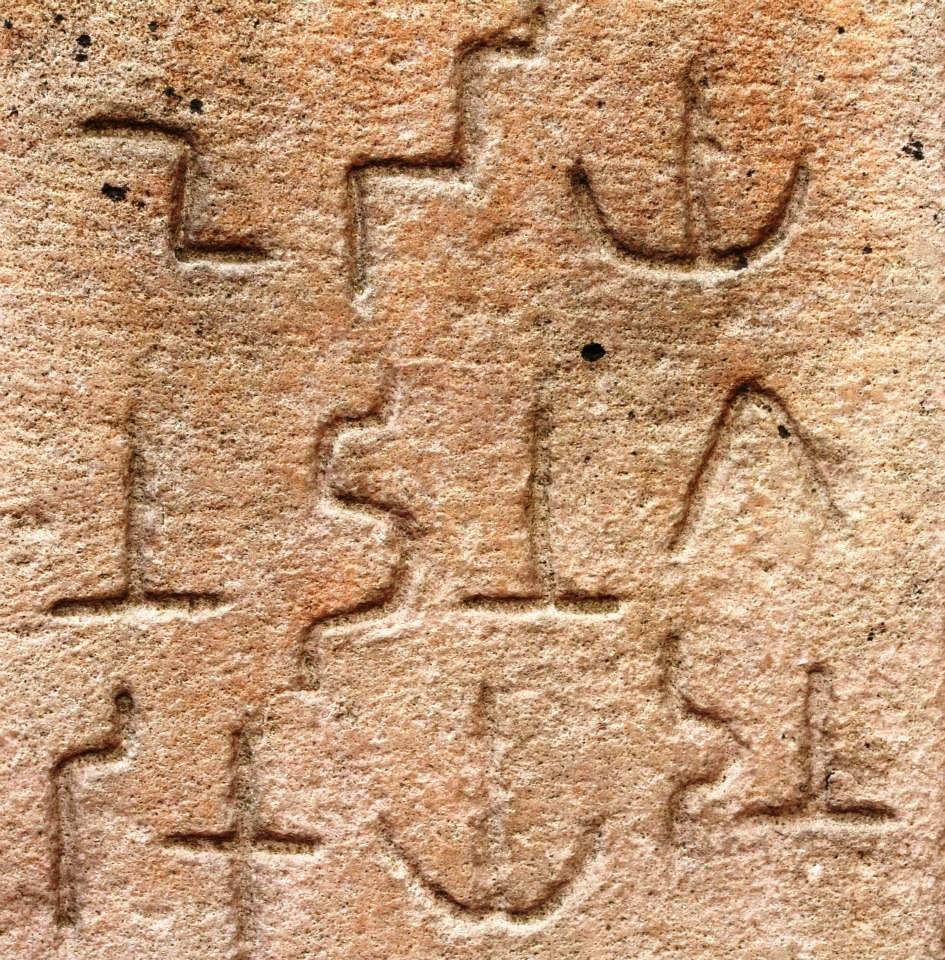
\includegraphics[scale=0.065]{"images/article-06/art06-fig01.jpg"}}

\textit{Example of Satavahana Brāhmī at Sanchi}

The Southern Gateway inscription by a foreman of artisans in Satavahana\index{Satavahana} king Satakarni’s\index{Satakarni} court on an architrave:

\vskip 4pt

\centerline{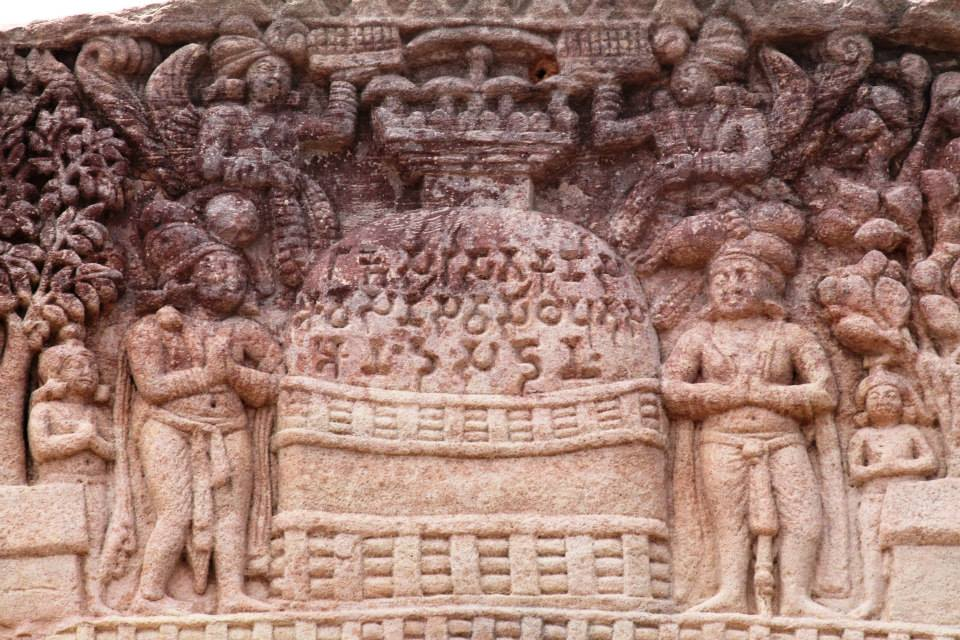
\includegraphics[scale=0.2]{"images/article-06/art06-fig02.jpg"}}

It reads:

Line 1 - Rano Siri Satakarnisa, Line 2 - avesanisavasithiputasa,\\ Line 3- Anamdasadanam

Donation of Vasithiputra Ananda, the foreman of the artisans of King Sri Satakarni

Satavahanas ruled from Pratishthanpur (today’s Paithan).

This is a typically inscribed in Satavahana Brāhmī\index{Satavahana Brahmi@Satavahana Brāhmī} style. This Brāhmī is now becoming curvy compared to angular style of Ashokan Brāhmī.\index{Ashokan Brahmi@Ashokan Brāhmī} Characters now have heads. Heads (lines) on present Nāgarī characters have apparent connection here. Interestingly, Satavahana Brāhmī was widely used south of Vindhya, in the areas ruled by Satavahanas.

\textit{Example of Gupta Brāhmī (widely accepted as pre-cursor to Nāgarī. script) at Sanchi:}

\vskip 3.5pt

\centerline{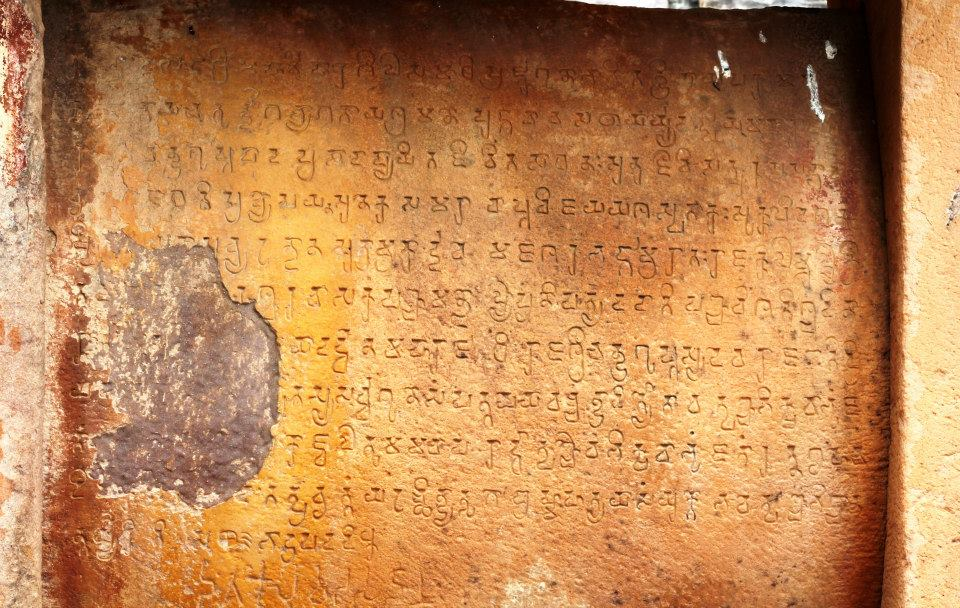
\includegraphics[scale=0.15]{"images/article-06/art06-fig03.jpg"}}

Here, the Brāhmī characters are becoming complete, curvy and have lines over them. Some letters can be instantly identified with Nāgarī.\index{Nagari@Nāgarī} characters. Gupta Brāhmī is also referred as Late Brāhmī and considered to be one of the earliest descendants of Brāhmī.\index{Brahmi@Brāhmī}

Sanchi was a meeting point of Indian writing traditions. We have seen examples of three distinct Brāhmī writing traditions, especially used by or identified with the emperor and mighty dynasties of India who ruled large swathe of India for long time.

We can also see some examples of Brāhmī and Nāgarī inscriptions together at Sanchi, E.g.,

\vskip 3pt

\centerline{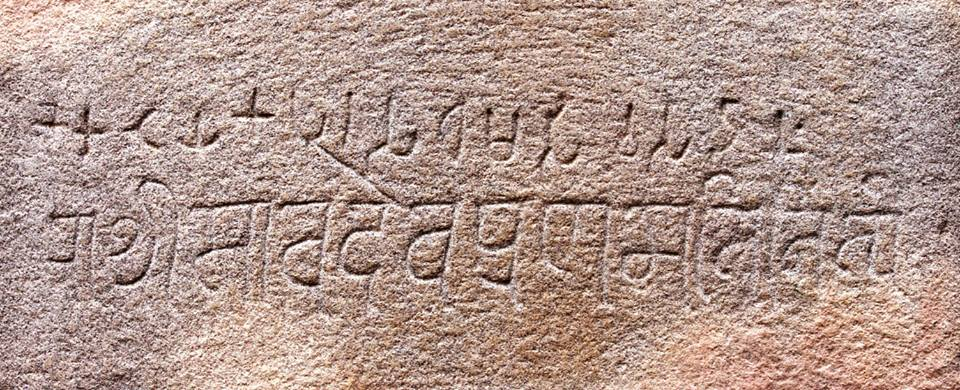
\includegraphics[scale=0.2]{"images/article-06/art06-fig04.jpg"}}

Or Standalone Nāgarī. example, e.g.,

\vskip 3pt

\centerline{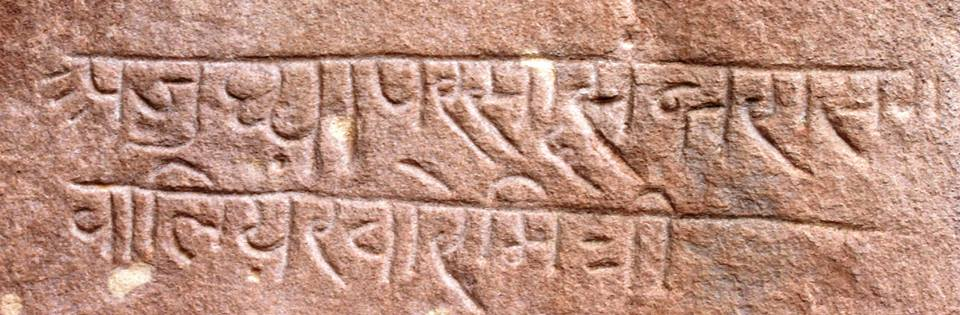
\includegraphics[scale=0.2]{"images/article-06/art06-fig05.jpg"}}

\textit{Kanheri Caves:}

Kanheri caves near Borivali house Brāhmī donative inscriptions, \textit{prashasti} and commemorative panels ranging from Ashokan Brāhmī\index{Ashokan Brahmi@Ashokan Brāhmī} of 1st Century BCE to very late Brāhmī of 7th/8th century. The Buddhist caves situated over here were Vihāras.\index{Viharas@Vihāras} These cave complex of 110+ caves was looking over the ancient routes connecting Sopara to the rest of Indian cities of trade importance; viz., Kalyan, Nasik, Junnar, Paithan, Ujjain etc.

It is believed that Kanehri\index{Kenehri} was university centre when the area was under the rule of Mauryas.\index{Maurya} The place is known to have remained active till 10th century CE.

Besides stone inscriptions numerous copper plates have been found at Kanheri. These copper plates are either inscribed with Brāhmī or Deva Nāgarī.\index{Deva Nagari@Deva Nāgarī} The number of Deva Nāgarī copper plates is higher. Most of the plates are found written in Sanskrit language.

\textit{Other Brāhmī Inscriptions}

The Ashokan edict discovered by Shri.\ Bhagwanlal Inderji at Sopara is the most outstanding example of Brāhmī found in this area. Sopara is 25 kms from Kanheri caves. This edict is currently housed at Chhatrapati Shivaji\index{Shivaji, Chhatrapati} Maharaj Vastu Sangrahalaya in Mumbai.

Nasik, Naneghat, Junnar are few of the important places where Brāhmī inscriptions are widely found, studied and recorded.

Further south, we have Ashokan rock edicts at Amaravati and at Yerragudi and Rajula-Mandagiri, near Pattikonda(Kurnool District); Sannati, Gulbarga district; and numerous major/minor edicts at Palkigundu and Gavimath in Koppal district, Karnataka, Suvarnagiri known as Kanakagiri in Koppal district, Brahmagiri, Chitradurga district, Rameshwara and Siddapur near Brahmagiri, Maski in Raichur district, Nittur and Udegolam in Bellary district.


\section*{Nāgarī\index{Nagari@Nāgarī} and Nandī Nāgarī\index{Nandi Nagari@Nandī Nāgarī} South of Vindhya}

Prima facie, the transition of Brāhmī to Nāgarī has happened almost simultaneously across the Bharat varsh in 9th -10th century. Nāgarī was as popular as Brāhmī in India, from today’s Afghanistan in the west / north west to Arakan in the east and to Sri Lanka in far south.

Before we look at them, the development of Nāgarī from Brāhmī is shown in the first table given below. Below the table of Nāgarī, a chart of Sharda script is given. The chart in the middle gives characters of Nandī Nāgarī, while the third chart shows characters of Grantha\index{Grantha script} and Tamil scripts. This looks like a big extended family and looking at the transition of each script, we find connection in strokes and curves amongst them. This is to understand similarity or ‘closeness’ with one another.

As understood from the tables, Nāgarī and Nandī Nāgarī looks almost the same barring certain characters. Keeping this in consideration, henceforth only ‘Nāgarī’ word will be used to denote both the scripts. Though many claim them to be sister scripts, Nandī Nāgarī looks to be a better claimant of modern Nāgarī.

Popularity and usage of Nāgarī and sister script (or mother script?) Nandī Nāgarī can be best understood by inscriptions and plates. However, a medium of exchange which is officially issued and widely used by common populace can be the best measure to understand the acceptability of a script or a language. A look at usage of Nāgarī on coinages will give perfect idea about spread and popularity of the script.

Various rulers south of Vindhya used the script on their precious and base metal coins. Use on base metal coin is significant as base metal coins were used by larger population, lower income strata labourers and sundry workers.

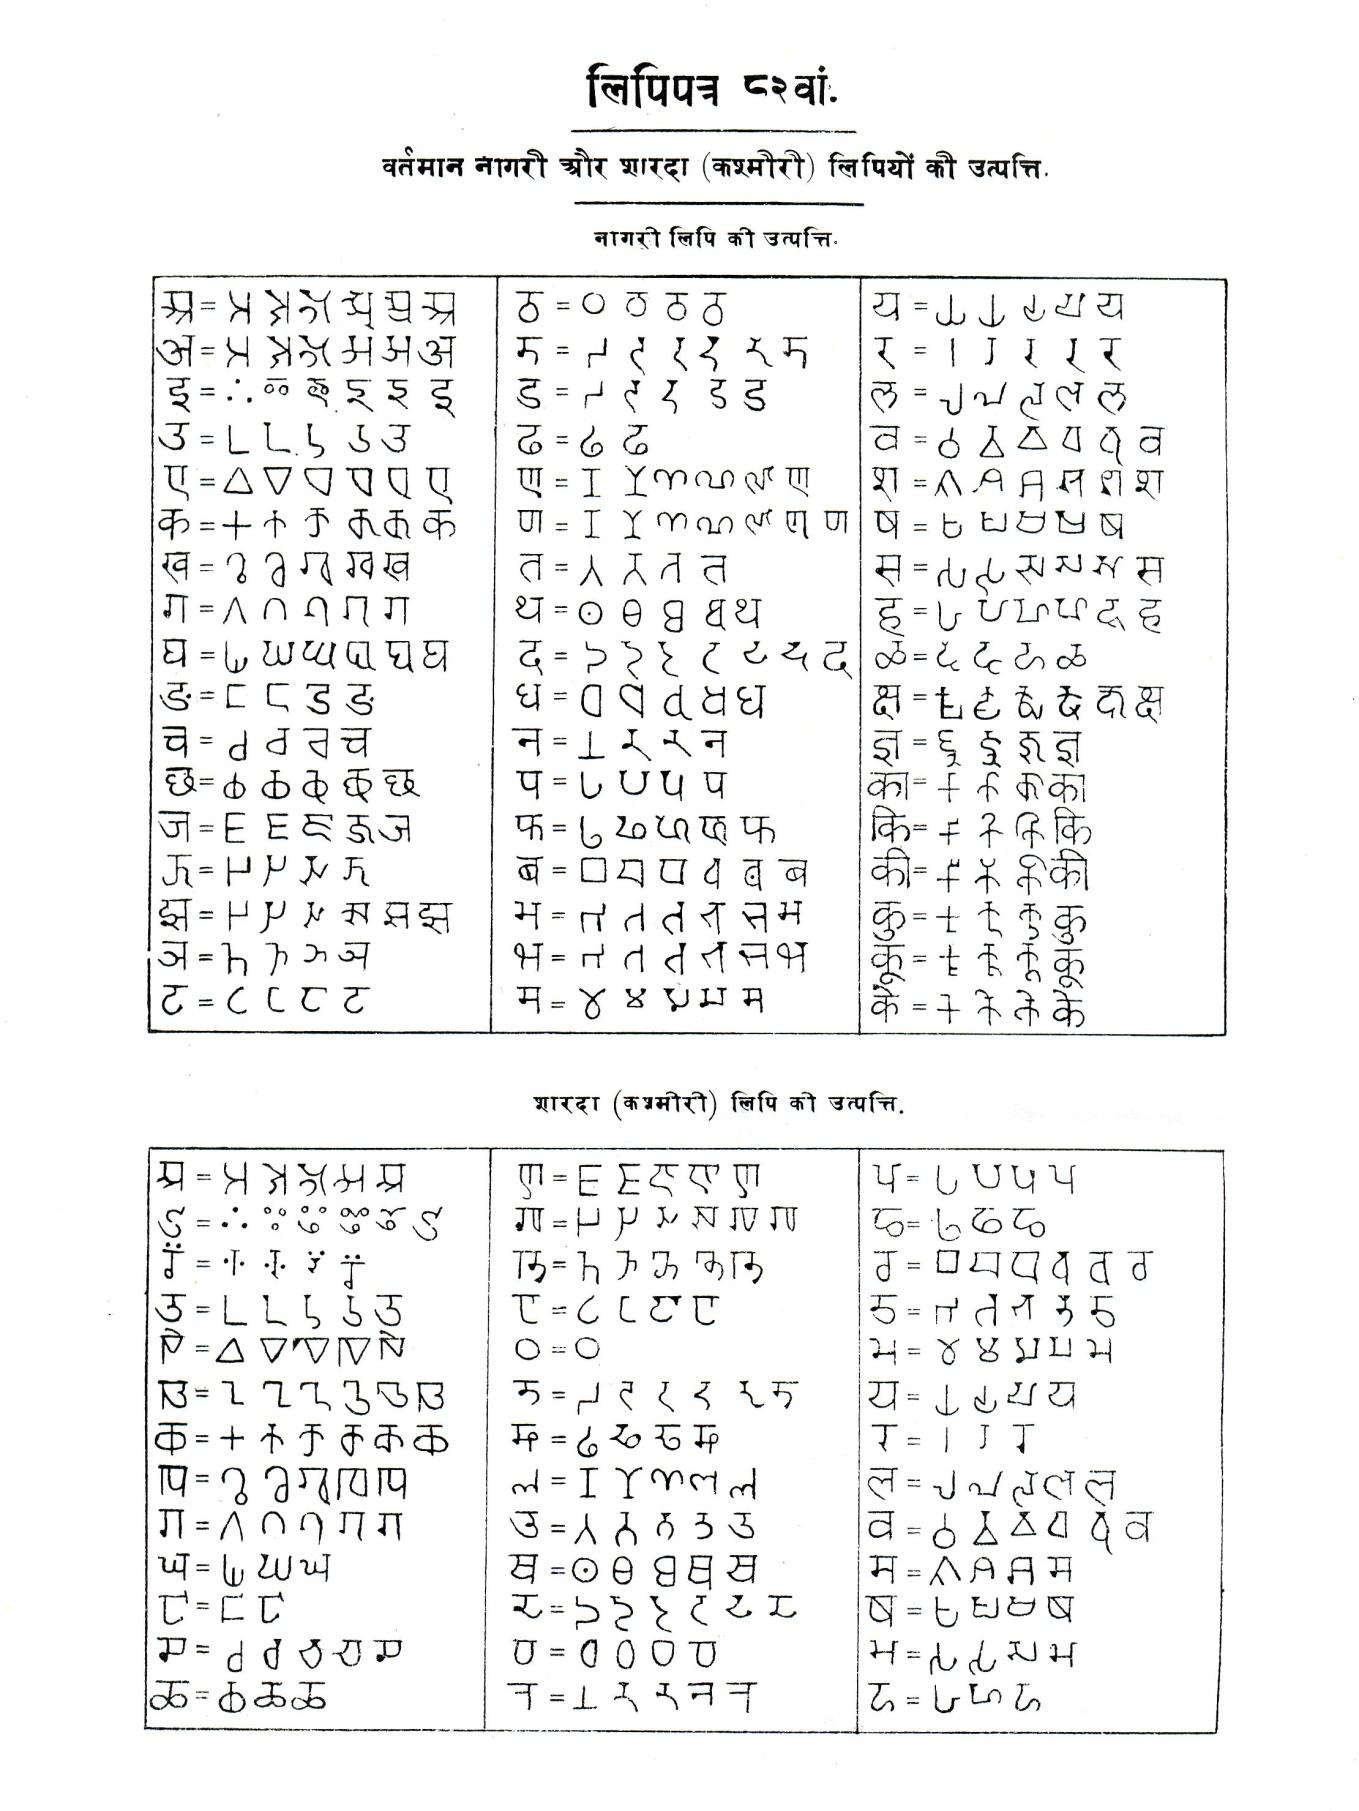
\includegraphics[scale=0.071]{"images/article-06/art06-fig06a.jpg"}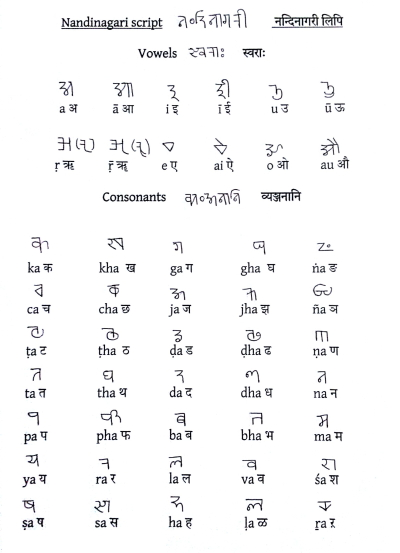
\includegraphics[scale=0.234]{"images/article-06/art06-fig06b.jpg"}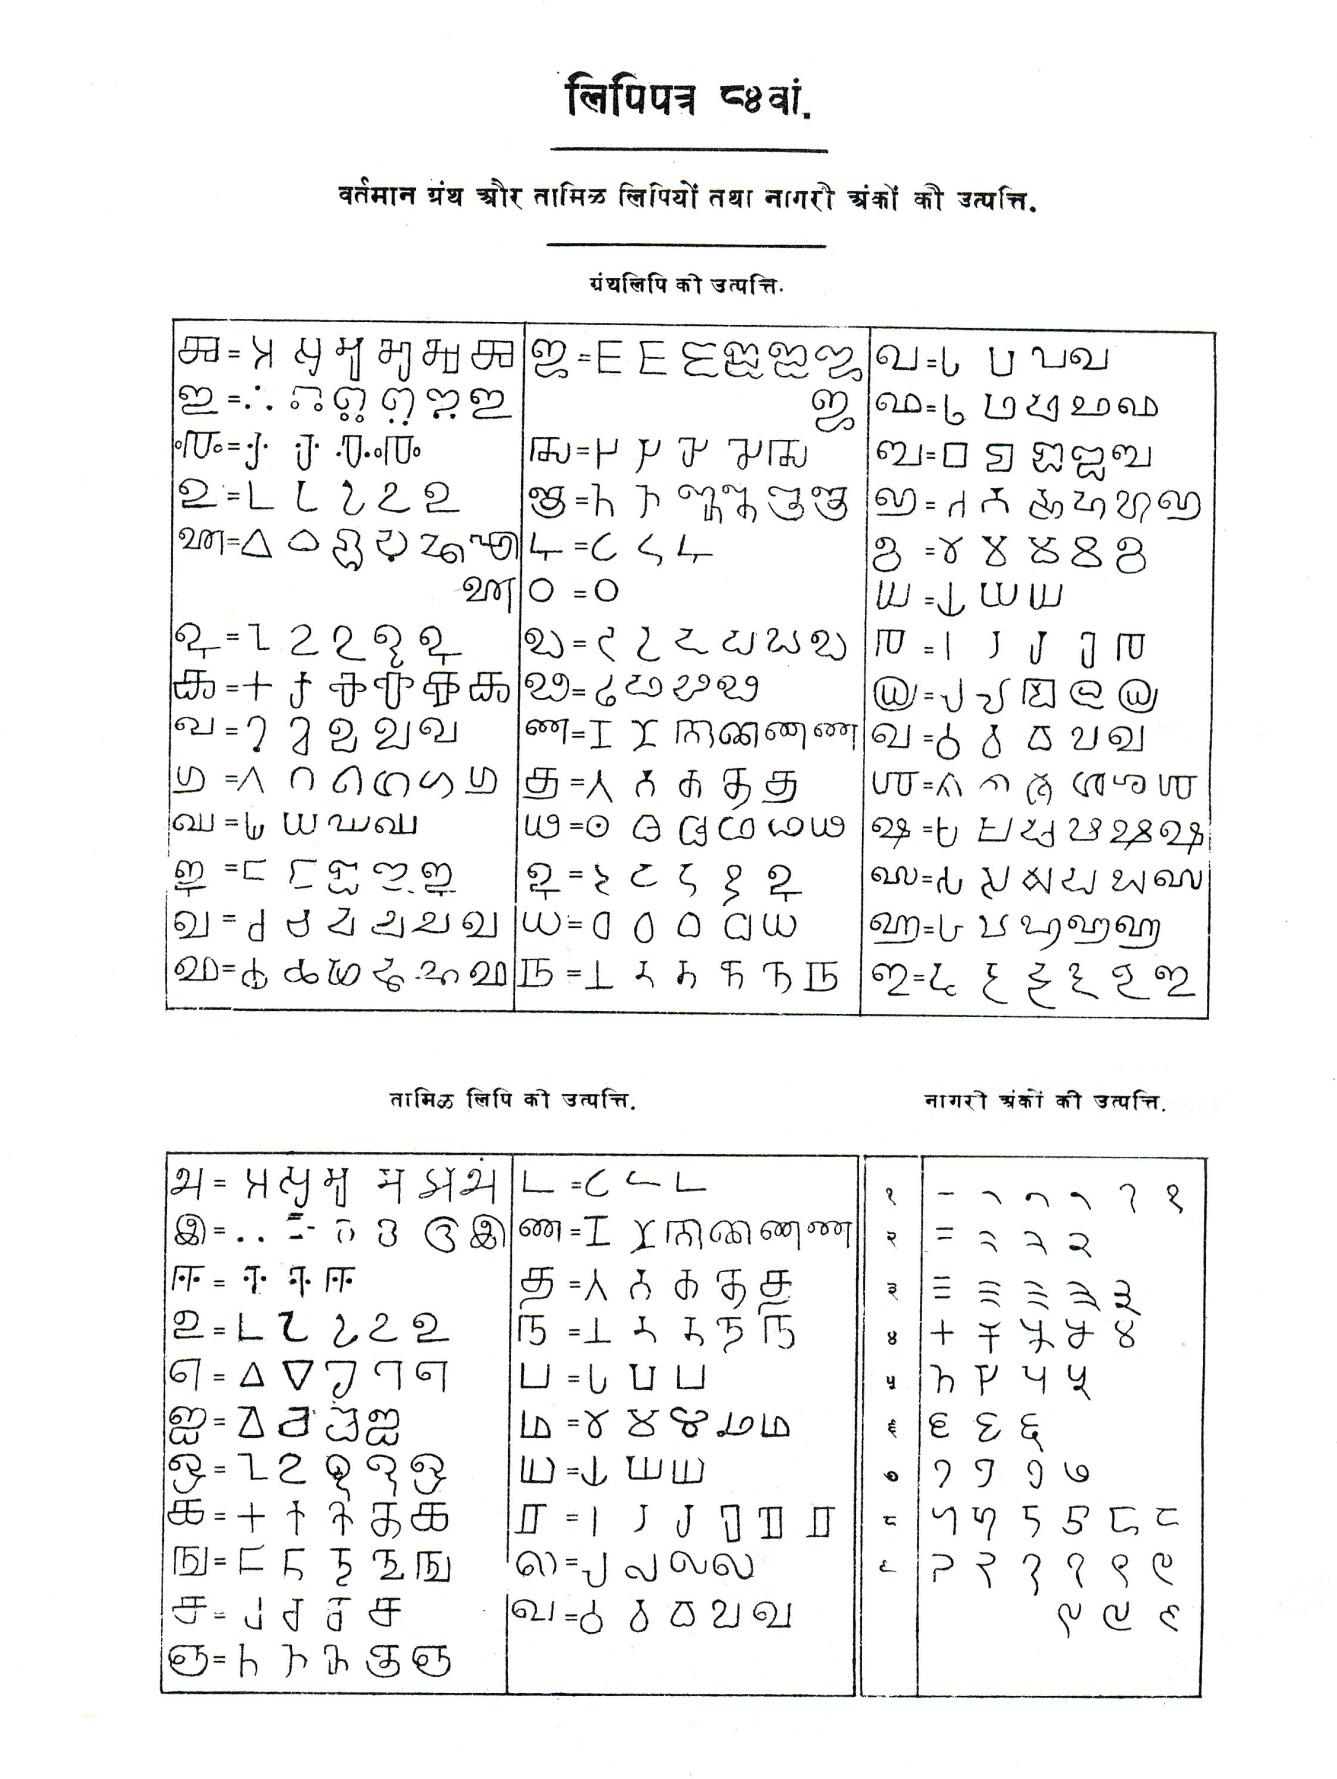
\includegraphics[scale=0.072]{"images/article-06/art06-fig06c.jpg"}

\subsection*{The Earliest Nāgarī and Nandī Nāgarī Inscriptions and use on coins}

Nāgarī remained in use for nearly a millennium in various empires, kingdoms and principalities south of Vindhya.

\textbf{Pallavas}

After the gradual disintegration of Satavahana\index{Satavahana} empire, Pallavas,\index{Pallava} who were feudatories of Satvahana rose to power in South India and ruled for nearly 500-600 years, from 3rd Century CE to 9th Century CE. Two kings – Mahendravarman\index{Mahendravarman} and Narsimhavarman\index{Narsimhavarman I} I are the most powerful amongst them. Pallava script (derived from Grantha script) was used as official script in their empire. As the other place around them were transitioning from Brāhmī and her derivatives to Nāgarī, Pallava ruler Narsimhavarman II’s inscription has been found inscribed with Nandī Nāgarī script, a script that has closeness to Nāgarī.

It is interesting to note that Pallava rulers used Brāhmī\index{Brahmi@Brāhmī} on their coins.\index{coins}

Narasimhavarman II, 700 - 728 CE, also known as Rajasimha Pallava,\index{Rajasimha Pallava} was a famous Pallava king, whose rule is seen as advancement in the field of literature and architecture. It is said that he himself has written works in Sanskrit.

\vskip 7pt

\centerline{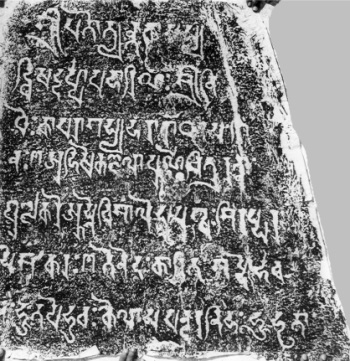
\includegraphics[scale=0.65]{"images/article-06/art06-fig07.jpg"}}

Narasimha Pallava’s Inscription in Nāgarī Script, 8th century C.E, Saluvankuppam, Mamallapuram, Tamil Nadu.

“The earliest Nāgarī charters in Tamil Nadu are the Paliyam copper plate inscriptions of the Ay king Varagunan (9th century CE).”

\url{http://www.tnarch.gov.in/epi/ins5.htm}

\textbf{Script of the Masses}

Two mighty empires south of Vindhya, the Cholas\index{Chola} and Vijayanagara\index{Vijayanagara} have minted coins in significantly large numbers bearing Nāgarī legend.


\subsection*{The Chola Dynasty}

The Chola\index{Chola} Dynasty was a Tamil dynasty that ruled primarily in Southern India.

Uttama Chola,\index{Uttama Chola} one of the rulers of the dynasty minted silver coins with legend Uttam / Chol in Nāgarī.

Uttama Chola was predecessor of illustrious emperor Raja Raja I.\index{Raja Raja I} His coins bears early Nāgarī. characters when it was almost in its early stage of development, some scholars call it a Proto-Nāgarī-phase.\index{Proto-Nagari-phase@Proto-Nāgarī-phase}

The letter Ma of Uttama resembles ‘Ma’ of Brāhmī almost completely.

Silver Kahavanu\index{Kahavanu} of Uttama Chola 970–985 CE:

\vskip 5pt

\centerline{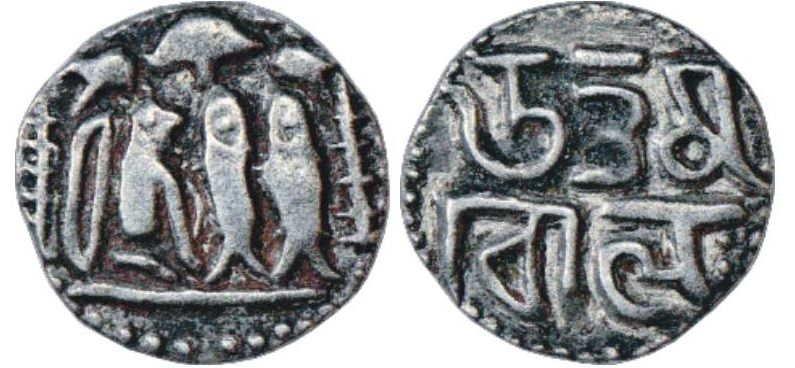
\includegraphics[scale=1.1]{"images/article-06/art06-fig08.jpg"}}

The obverse of the coin depicts a tiger seated right, an umbrella and a pair of upright fish. The reverse bears Nāgarī legend ‘Uttama/ Chola’.

Mighty imperial Chola emperors, especially Rajaraja I and Rajendra I minted coins in copper, silver and gold with legends in Nāgarī script.

Here is a gold fanam of Raj Raja I 985-1014 CE, with title Yuddha Malla.\index{Yuddha Malla} Under his rule the Chola empire expanded with his rule stretching from Kalinga to Sri Lanka. Raja Raja I\index{Raja Raja I} was one of the greatest rulers of the Chola Dynasty and he adopted the title “Yudhha Malla” which means victorious in battlefield or war, and the same title was depicted on his gold coins:

\vskip 4pt

\centerline{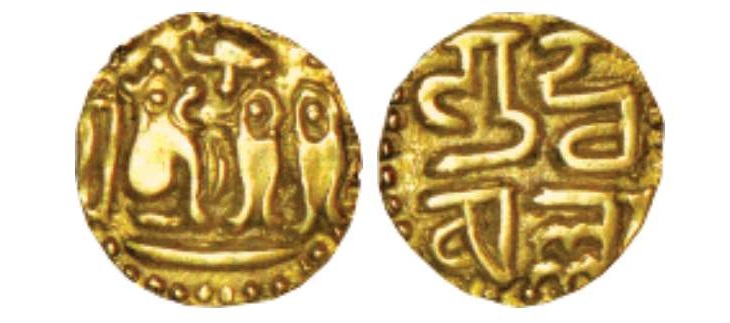
\includegraphics[scale=0.95]{"images/article-06/art06-fig09.jpg"}}

Gold Kahavanu\index{Kahavanu} of Raj Raja Chola with Nāgarī legend Gangaikonda Chola\index{Gangaikonda Chola} or the “conqueror of the Ganga valley” on obverse as well as reverse is depicted below. Proto-Nāgarī characters in the imperial coins speak more about the popularity of the script since such coins are also available in silver and copper:

\vskip 4pt

\centerline{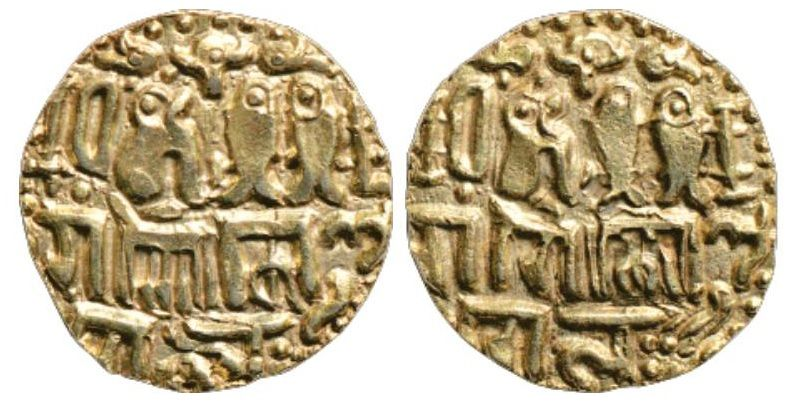
\includegraphics[scale=1]{"images/article-06/art06-fig10.jpg"}}

Base Gold Kahavanu of Raj Raja Chola with legend Raja Raja in Nāgarī:

\vskip 4pt

\centerline{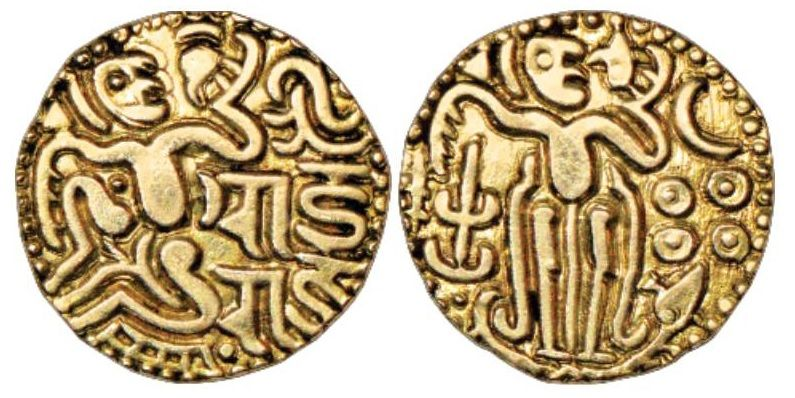
\includegraphics[scale=1]{"images/article-06/art06-fig11.jpg"}}

Copper Kahavanu\index{Kahavanu} of Raj Raja Chola with the legend Gangaikonda Chola on obverse and reverse. The design of gold, base gold and copper coins bear the same legend while weight is different:

\centerline{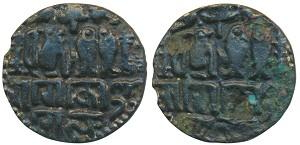
\includegraphics[scale=0.6]{"images/article-06/art06-fig12.jpg"}}

Gold Kahavanu of Rajendra Chola 1012-1044 CE with Nāgarī Legend Shri.\ Rajendra on obverse as well as reverse:

\centerline{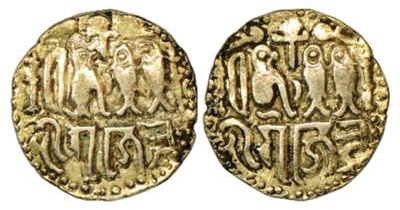
\includegraphics[scale=0.45]{"images/article-06/art06-fig13.jpg"}}

Ceylon man type gold Kahavanu\index{Kahavanu} of Rajadhiraja Chola\index{Rajadhiraja Chola} – 1044-1054 CE with Nāgarī legend Raja /Dhira/ Ja on obverse:

\centerline{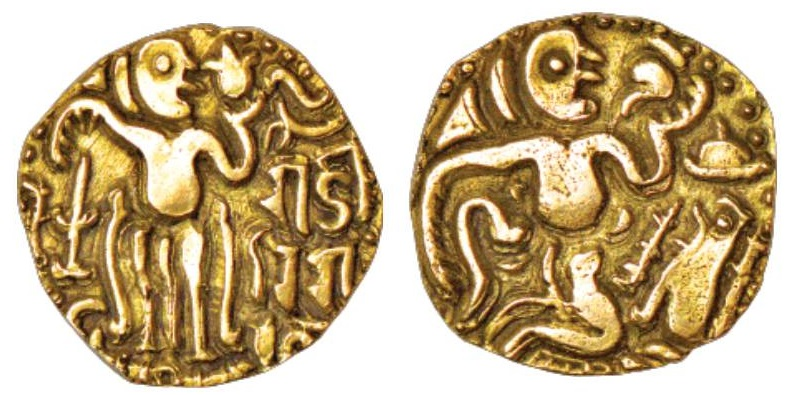
\includegraphics[scale=0.45]{"images/article-06/art06-fig14.jpg"}}

Before looking at Vijayanagar empire’s coinages for the usage of Nāgarī, a glance at some of the kingdoms and principalities where Nāgarī was popular and widely used in administration and their coinages.


\subsection*{The Alupa-s\index{Alupas} of Coastal Karnataka}

Alupa or Alva dynasty ruled in Tulunadu region of Coastal Karnataka from 200-450 CE. They became feudatories of Kadambas\index{Kadamba} of Banavasi, then of Chaulukya,\index{Chaulukya} Rashtrakuta,\index{Rashtrakuta} Hoysala\index{Hoysala} and later of Vijayanagar\index{Vijayanagara} empire.

Gold Pagoda of an Alupa ruler with title Shri.\ Pandya Dhananjaya\index{Dhananjaya, Shri. Pandya} legend in Nāgarī, attributed to period 1088-1332

\vskip 3pt

\centerline{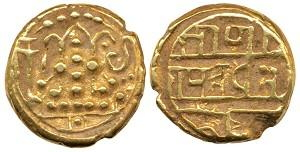
\includegraphics[scale=0.53]{"images/article-06/art06-fig15.jpg"}}

Alupa rulers minted coins with Nāgarī\index{Nagari@Nāgarī} legend for centuries. They also minted coins with Kannada legend simultaneously.

\textit{Coinage of Kadamba-s of Goa}

Gold pagodas with Nāgarī script are found in plenty from 11th century to early 13th century. They ruled from Goppakkapattan, ancient port of the present day Goa. They helped Chaulukyas to defeat Rashtrakuta. Language of Kadamba\index{Kadamba} administration was Sanskrit and Kannada\index{Kannada} while coins were inscribed with Nāgarī legend.

Gold pagoda of Shiva Chitta\index{Chitta, Shiva} with Nāgarī legend:

\vskip 3pt

\centerline{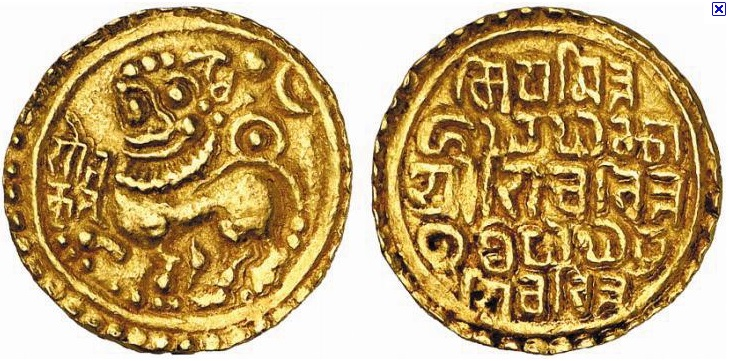
\includegraphics[scale=0.6]{"images/article-06/art06-fig16.jpg"}}

\textit{Yadavas\index{Yadava} of Devagiri}

Yadavas of Devagiri ruled from their capital Devagiri – the present day Daulatabad. They ruled the regions North Karnataka and Maharashtra upto present day Madhya Pradesh from 9th to 14th Century CE. They were patrons of Kannada\index{Kannada} and Sanskrit\index{Sanskrit literature} literature. Their coinages are inscribed with Nāgarī legend.

Silver Kasu\index{Kasu} of Yadava ruler Seundeva:\index{Seundeva}

\vskip 3pt

\centerline{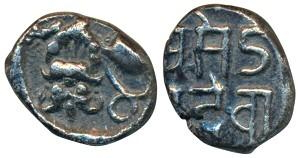
\includegraphics[scale=0.7]{"images/article-06/art06-fig17.jpg"}}

Gold Padma Tanka\index{Tanka, Padma} of Mahadeva, with Mahadeva\index{Mahadeva} in Nāgarī:

\centerline{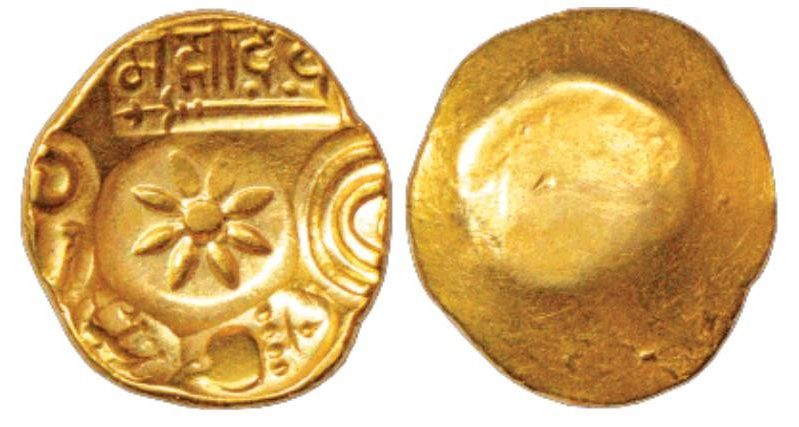
\includegraphics{"images/article-06/art06-fig18.jpg"}}


\section*{Coinage of Vijayanagara\index{Vijayanagara} Empire}

Two hundred years of coinages minted have innumerable varieties of gold, silver and copper with Nāgarī legend inscribed on them. After Chola\index{Chola} empire, this is another empire which had prolific coinages meant for every class of the society and economic transactions with fractions as small as 0.11 gram in silver to double pagoda as heavy as 7.8 gram in gold.

Silver Tara weighing 0.26g of Hari Hara II 1377-1404 CE:

\vskip 2pt

\centerline{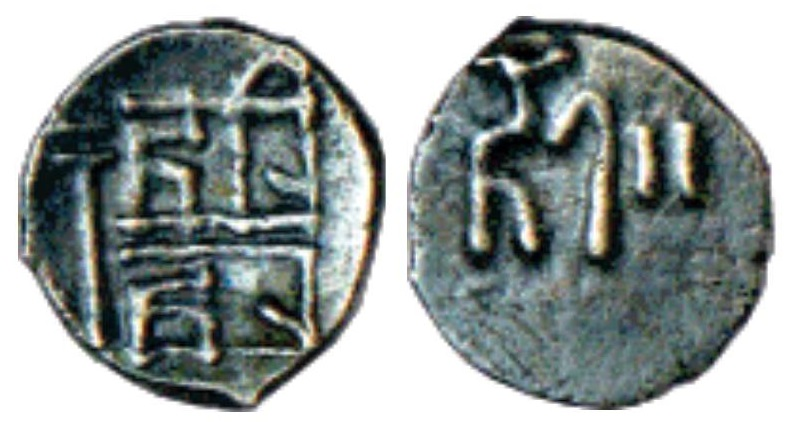
\includegraphics[scale=0.47]{"images/article-06/art06-fig19.jpg"}}

Gold Double pagoda weighing 7.8g of Shri.\ Krishna Devaraya\index{Devaraya, Shri. Krishna} 1509-1529 CE:

\centerline{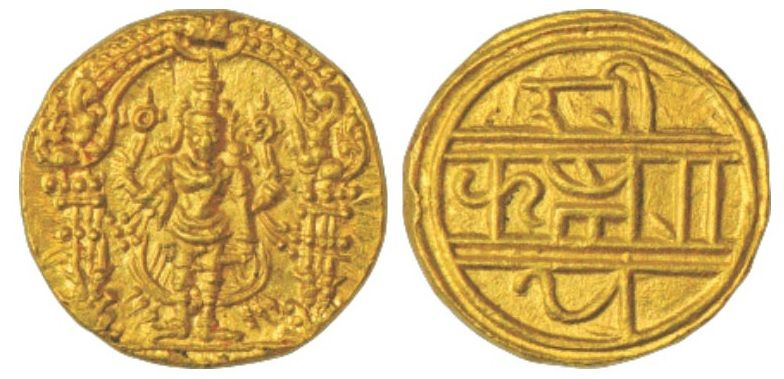
\includegraphics[scale=0.37]{"images/article-06/art06-fig20.jpg"}}


\subsection*{Other interesting coins of Vijayanagara Empire}

Gold Fanam of Sadasiva Raya\index{Raya, Sadasiva} with clear Nāgarī Sa on Reverse:

\vskip 4pt

\centerline{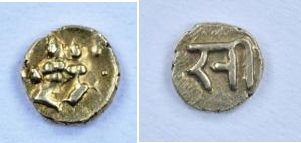
\includegraphics[scale=0.6]{"images/article-06/art06-fig21.jpg"}}

Gold Half-Fanam of Devaraya II with Shri.\ Pratapa Raya\index{Raya, Shri. Pratapa} in DevaNāgarī:

\vskip 4pt

\centerline{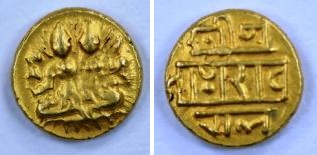
\includegraphics[scale=0.6]{"images/article-06/art06-fig22.jpg"}}

Copper Unit of Shri.\ Krishna Deva Raya, Tamil Nadu Series with legend in Nāgarī – Shri.\ Pra/Tapa Krishna/Raya:

\vskip 4pt

\centerline{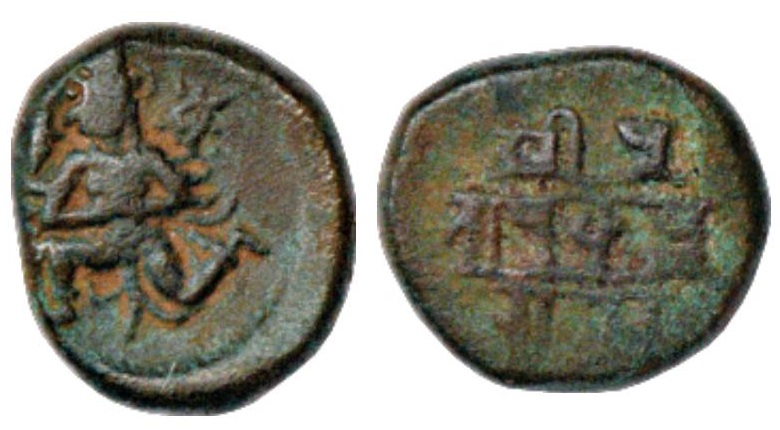
\includegraphics[scale=0.5]{"images/article-06/art06-fig23.jpg"}}

After the disintegration of Vijayanagar empire, many small rulers, mostly Nayakas of different regions minted coins with Nāgarī legend. These coins are found in all three metals and in many varieties.

Chhatrapati Shivaji\index{Shivaji, Chhatrapati} Maharaj also minted coins in all three metals with Deva Nāgarī\index{Deva Nagari@Deva Nāgarī} legend. After Marathas aligned with Mughals, the coinage of Peshwas\index{Peshwas} were mainly inscribed with Persian with occasional Nāgarī words used which were very few. Nāgarī almost disappeared from South Indian coinage in late 19th Century with few exceptions.

Entire history of the Bhonsle kings\index{Bhonsle kings} of Thanjavur has been engraved, at the instance of Serfoji II,\index{Serfoji II} (1798-1837) the Maratha king of Thanjavur, on the walls of the Brihadishwar temple\index{Brihadishwar temple} in Nāgarī.

With Geroge V’s base metal coins (1911-1937 CE), Nāgarī words were again inscribed, though along with other scripts, in 8/4/2 anna coins. They remained to be used in small fraction even during the reign of George VI. After the independence, Roman characters share space with Nāgarī\index{Nagari@Nāgarī} on Indian coinage, and now we have bi-lingual/bi-scriptual coins.

This is the journey of Nāgarī in various kingdoms and empires south of Vindhya range. Nāgarī, though derived from Brāhmī, along with other Brāhmī\index{Brahmi@Brāhmī} derived scripts, became main stream and used for 1000+ years on a medium of exchange be it of gold or copper or other base metal. Nāgarī still remains strong in 21st century.

There are many Nāgarī inscriptions found across the states and regions discussed here. However, coinages as evidence carry more weight since it reaches each and everyone in the society, cross the border and travels far away, preserved and sometimes land in the hands of numismatists to tell various stories. One story is about a script that replaced Brāhmī as common script of Bharatavarsha, of Indian people shattering some beliefs peddled to convince people of this country that there was no single script in India.


\subsection*{Nāgarī’s Travel further South to Sri Lanka}

With Cholas conquering Sri Lanka,\index{Sri Lanka} Nāgarī was introduced on its coinages and remained in use for a long time. Brāhmī, was once used widely in Sri Lanka and now was replaced by Nāgarī.

Vijayabahu I\index{Vijayabahu I} who ended Chola rule in Sri Lanka, Parakrama Bahu,\index{Parakrama Bahu} the monarch issued coins with legend Shri.\ Parakram Bahu in Nāgarī.

All the scripts of India including that of Tibet are Brāhmīc Scripts. As mentioned earlier, Gupta Brāhmī (4-5th Century CE) is precursor to modern Nāgarī, known as Late Brāhmī script went beyond Gupta hold and went North-west upto today’s Afghanistan, East-North-East upto Arakan to Sri Lanka in the south of South India and Upto Sindh/Gujarat in the west and became a Pan-Indian Script, though in various forms and known by various names. It was a redux of Pre-Gupta Brāhmī going Pan-Indian in various forms which was used right beyond Afghanistan to Burma to Sri Lanka and Sindh/Gujarat.

To Afghanistan:

\vskip 5pt

\centerline{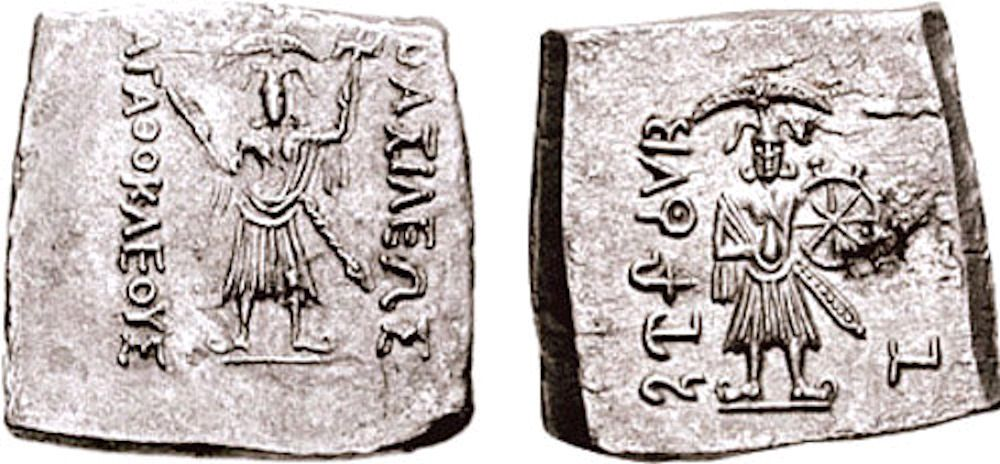
\includegraphics[scale=0.95]{"images/article-06/art06-fig24.jpg"}}

Coin of Indo-Greek ruler Agathokleyas\index{Agathokleyas} 190-180 BE with Brāhmī legend Rajane Agathukleyasa along with Lord Sri Krishna standing with Chakra (reverse), on obverse Balarama\index{Balarama} with Plough, Greek legend on both sides. Eventually this is one of the earliest depiction of Lord Krishna and Balarama on coin, significant as these coins were found at Al Khanoum, Afghanistan.

After nearly thousand years, Hindu Shahis or Kabul Shahis of Afghanistan used Nāgarī on their coins. This is western boundary of Nāgarī as well. The eastern boundary of Nāgarī can be traced to \index{Arakan} region and the southern- most to Sri Lanka.


\section*{Conclusion}

The above amply proves how the whole nation was connected Pre- 900 CE by Brāhmī and Post- 900 CE by Nāgarī script.

This puts the belief to rest that India was never integrated by one language or one script. India, in fact, was a garland of precious / semi-precious stones, pearls and exotic beads tied together by threads of shared culture, languages and common script/s.

All Sanchi images’ photography by – Bimal Trivedi

\newpage


\section*{Bibliography}

\begin{thebibliography}{99}
\itemsep=2pt
\bibitem{chap6-key01} Girijapathi, M. \textit{The Coinage and History of Vijayanagar Empire}

 \bibitem{chap6-key02} Mitchiner, Michael. \textit{The Early Indo-Greeks and Their Antecedants}

 \bibitem{chap6-key03} Oza, G. H. \textit{Prachin Bharatiya Lipimala}

 \bibitem{chap6-key04} Patel, Purushottam G.; Pandey, Pramod; Rajgor, Dilip (2007). \textit{The Indic Scripts: Palaeographic and Linguistic Perspectives}. D.K. Printworld. ISBN 978-81-246-0406-9.

 \bibitem{chap6-key05} Ray, Niharranjan (1993). \textit{Bangalir Itihas: Adiparba in Bengali}. Calcutta: Dey's Publishing, ISBN 81-7079-270-3, p. 59

 \bibitem{chap6-key06} Salomon, Richard (1998). \textit{Indian Epigraphy: A Guide to the Study of Inscriptions in Sanskrit, Prakrit and the Other Indo-Aryan Languages}. Oxford: Oxford University Press. ISBN 0-19-509984-2.

 \bibitem{chap6-key07} “A Note on Inscriptions in Bombay". \textit{Maharashtra State Gazetteers-Greater Bombay District}. Government of Maharashtra. 1986. Retrieved 2012-11-23. \url{https://cultural.maharashtra.gov.in/english/gazetteer/greater_bombay/inscriptions.html}

 \bibitem{chap6-key08} \url{www.classicalnumismaticgallery.com}

 \bibitem{chap6-key09} \url{www.todywallaauctions.com}

 \bibitem{chap6-key10} \url{http://coins.lakdiva.org/ruhuna/ruhuna_floral_Brāhmī_pb.html}

 \bibitem{chap6-key11} \url{https://en.wikipedia.org/wiki/Tissamaharama_Tamil_Brāhmī_inscription}

 \bibitem{chap6-key12} \url{https://en.wikipedia.org/wiki/Pyu_script}

 \bibitem{chap6-key13} \url{http://www.frontline.in/static/html/fl2013/stories/20030704000207100.htm}

 \bibitem{chap6-key14} Kerala Brāhmī Example: \url{http://www.thehindu.com/news/national/kerala/newly-discovered-Brāhmī-inscription-deciphered/article5777862.ece}, E M Manoj, MARCH 12, 2014

 \end{thebibliography}

